\section{Tiến hành thí nghiệm}

Các bước thí nghiệm chung:

\begin{enumerate}
    \item Thêm nhiễu cho ảnh bằng MATLAB
    \item Xử lý nhiễu bằng MATLAB trên máy tính và xứ lý nhiễu bằng Python trên Raspberry Pi 3
    \item Lấy kết quả MATLAB làm chuẩn để đánh giá kết quả giảm nhiễu ảnh trên Raspberry Pi.
\end{enumerate}

\begin{figure}[H]
    \centering
    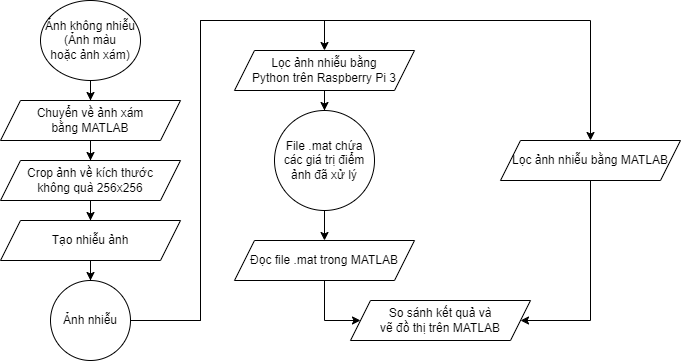
\includegraphics[width=\linewidth]{../images/denoise_flowchart.png}
    \caption{Quy trình thí nghiệm}
\end{figure}

Để đánh giá hiệu quả của bộ lọc, ta tính sai số bình phương trung bình (mean square error, MSE) giữa ảnh gốc và ảnh đã lọc:

\begin{equation}\label{eqn:MSE}
    MSE = \frac{1}{WH} \sum_{i=1}^{H} \sum_{j=1}^{W} {(y_{ij} - x_{ij})^2}
\end{equation}

Trong đó, $W$ và $H$ là chiều rộng và chiều cao ảnh, $x$ là ảnh gốc và $y$ là ảnh đã lọc.

Ta tìm MSE bằng hàm \verb|mse| có sẵn của MATLAB.

\subsection{Lọc nhiễu ảnh muối tiêu}

\subsubsection{Tạo ảnh nhiễu muối tiêu trên MATLAB}

Ta đọc một ảnh gốc (ảnh màu hoặc ảnh xám), chuyển sang ảnh xám nếu cần, crop ảnh xuống $256 \times 256$ để thuận tiện cho việc xử lý. Cuối cùng, ta tạo nhiễu muối tiêu cho ảnh bằng hàm \texttt{imnoise} có sẵn của MATLAB.

\begin{lstlisting}[language=MATLAB]
figure, tiledlayout(1,2)

% Doc anh, chuyen sang anh xam, va crop anh neu kich thuoc lon hon 255
I = imread('dataset\4.1.03.tiff');
I = rgb2gray(I);
[rows, cols] = size(I);
size = [rows, cols];
if (rows > 256), I = imresize(I, [256 NaN]), end;
if (cols > 256), I = imresize(I, [NaN 256]), end;

% Luu anh xam da crop va hien thi anh
imwrite(I, '../images/salt_pepper_orig.bmp')
nexttile, imshow(I), title('Anh goc')

% Them nhieu muoi tieu voi mat do 0.05
J = imnoise(I, 'salt & pepper', 0.05);

% Luu anh da duoc tao nhieu va hien thi anh
imwrite(J, '../images/salt_pepper_noise.bmp')
nexttile, imshow(J), title('Anh nhieu muoi tieu 5%')
\end{lstlisting}

\begin{figure}[H]
    \centering
    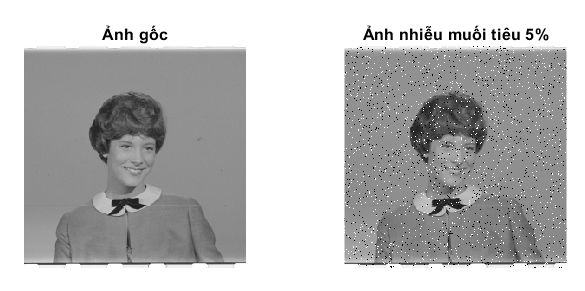
\includegraphics[width=.75\linewidth]{../images/salt_pepper_noise_matlab.png}
    \caption{Tạo ảnh nhiễu muối tiêu trên MATLAB}
\end{figure}

\subsubsection{Lọc ảnh nhiễu muối tiêu bằng Python trên Raspberry Pi 3}

Các bước triển khai hàm lọc trung vị kích thước $3 \times 3$ trên Python như sau (Hình \ref{fig:median_filtering_algorithm}):

\begin{itemize}
    \item Padding cho ngõ vào: Để không bỏ sót các điểm ảnh ở rìa, ta cần padding cho ảnh ngõ vào. Vì bộ lọc có kích thước 3x3, ta cần padding 1 hàng zero cho rìa trên và dưới, và padding 1 cột zero cho rìa trái và phải.

    \item Tìm trung vị: Cho vòng lặp chạy qua từng điểm ảnh. Ở mỗi vòng lặp, xếp các điểm ảnh lân cận vào một mảng, sắp xếp mảng theo thứ tự tăng dần (hoặc giảm dần), và điểm ảnh ngõ ra sẽ là phần tử ở giữa của mảng đã sắp xếp.
\end{itemize}

\begin{figure}[H]
    \centering
    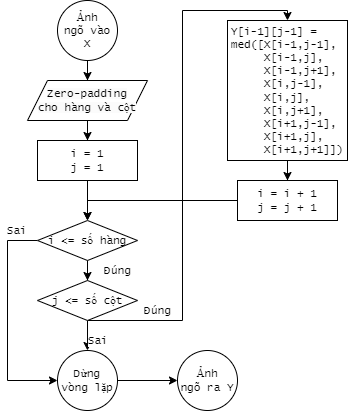
\includegraphics[width=.5\linewidth]{../images/median_filtering_algorithm.png}
    \caption{Thuật toán lọc trung vị}
    \label{fig:median_filtering_algorithm}
\end{figure}

\begin{lstlisting}[language=Python]
import cv2
import numpy as np
import matplotlib.pyplot as plt
import scipy.io

# Doc anh nhieu muoi tieu
I = cv2.imread('output/salt_pepper_noise.png', cv2.IMREAD_GRAYSCALE)

# Ham loc trung vi kich thuoc 3x3
def medFilter3x3(X):
  nRows, nCols = X.shape

  # Padding cho anh ngo vao
  hpad = np.zeros((1, nCols))
  X = np.vstack((hpad, X, hpad))
  vpad = np.zeros((nRows+2, 1))
  X = np.hstack((vpad, X, vpad))
  
  # Lay trung vi bang cach sap xep theo thu tu lon dan
  # va chon phan tu thu 5 trong 9 phan tu
  Y = np.zeros((nRows,nCols))
  for i in range(1,nRows+1):
    for j in range(1,nCols+1):
      x = [X[i-1,j-1],
           X[i-1,j],
           X[i-1,j+1],
           X[i,j-1],
           X[i,j],
           X[i,j+1],
           X[i+1,j-1],
           X[i+1,j],
           X[i+1,j+1]]
      x = sorted(x)
      Y[i-1][j-1] = x[4]
  return Y

# Loc trung vi voi bo loc 3x3
J = medFilter3x3(I)

# Luu ket qua theo dinh dang cua MATLAB
scipy.io.savemat('output/salt_pepper_denoised_rpi3.mat', {"rpiDenoisedImg": J})
\end{lstlisting}

Kết quả chạy chương trình trên Raspberry Pi 3: 
Chương trình đọc ảnh nhiễu ngõ vào và xuất file \verb|salt_pepper_denoised_rpi3.mat| thành công để đưa vào MATLAB.

\subsubsection{So sánh kết quả với MATLAB}

Ta lọc ảnh bằng bộ lọc trung vị kích thước $3 \times 3$ với hàm \texttt{medfilt2()} có sẵn của MATLAB. 
Tiếp đến, ta vẽ ảnh đã lọc từ MATLAB và từ Raspberry Pi 3, 
đồng thời đánh giá các kết quả này dựa trên sai số bình phương trunb bình giữa ảnh đã lọc và ảnh gốc.

\begin{lstlisting}[language=MATLAB]
figure
tiledlayout(1,4)

% Doc anh xam goc va hien thi
I = imread('../output/salt_pepper_orig.png');
nexttile, imshow(I), title('Anh goc')

% Doc anh nhieu muoi tieu va hien thi
J = imread('../output/salt_pepper_noise.png');
nexttile, imshow(J), title('Anh nhieu muoi tieu')

% Loc trung vi voi bo loc 3x3 bang ham co san va hien thi
K = medfilt2(J, [3 3]);
nexttile, imshow(K), title(["Loc trung vi 3x3", "(MATLAB)"])
imwrite(K, '../output/salt_pepper_denoised_matlab.png')

% Doc ket qua loc trung vi 3x3 tu Raspberry Pi 3 va hien thi
load('../output/salt_pepper_denoised_rpi3.mat')
L = uint8(rpiDenoisedImg);
nexttile, imshow(L), title(["Loc trung vi 3x3", "(RPi 3)"])
imwrite(L, '../output/salt_pepper_denoised_rpi3.png')

% Sai so binh phuong trung binh giua anh goc va anh da loc
fprintf('MSE (MATLAB): %.4f\n', mse(I, K));
fprintf('MSE (RPi 3): %.4f\n', mse(I, L));
\end{lstlisting}

Kết quả chạy:

\begin{lstlisting}[style=output]
MSE (MATLAB): 3.8137
MSE (RPi 3): 3.8137
\end{lstlisting}

\begin{figure}[H]
    \centering
    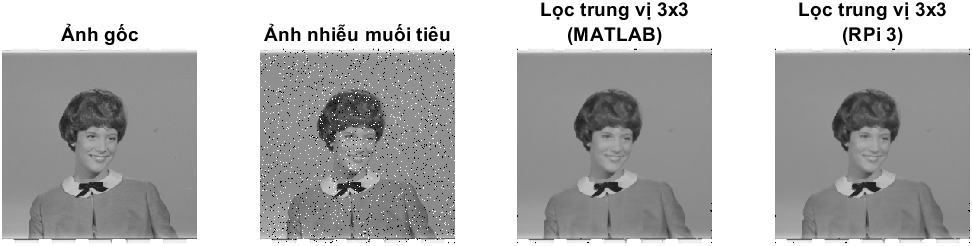
\includegraphics[width=1\linewidth]{../images/salt_peper_compare.png}
    \caption{So sánh kết quả lọc trung vị từ Raspberry Pi 3 so với MATLAB}
\end{figure}

\textbf{Nhận xét:} Kết quả lọc trung vị từ Python trên Raspberry Pi hiệu quả tương đương MATLAB. 
Sai số bình phương trung bình giữa ảnh gốc và ảnh đã lọc trên Raspberry Pi 3 và trên MATLAB là giống nhau.

\subsubsection{So sánh trên toàn bộ dữ liệu}

Thực hiện cùng quy trình thí nghiệm này với các ảnh còn lại trong bộ dữ liệu, ta thu được kết quả sau:

\begin{table}[H]
\centering
\begin{tabular}{|c|c|c|}
\hline
\textbf{Filename} & \textbf{MATLAB} & \textbf{RPi 3} \\ \hline
4.1.01 & 9.2762 & 9.2762 \\ \hline
4.1.02 & 9.8379 & 9.8379 \\ \hline
4.1.03 & 3.8523 & 3.8523 \\ \hline
4.1.04 & 5.6225 & 5.6225 \\ \hline
4.1.05 & 9.2456 & 9.2456 \\ \hline
4.1.06 & 24.7663 & 24.7663 \\ \hline
4.1.07 & 3.1220 & 3.1220 \\ \hline
4.1.08 & 3.9775 & 3.9775 \\ \hline
4.2.01 & 4.3840 & 4.3840 \\ \hline
4.2.03 & 40.0398 & 40.0398 \\ \hline
4.2.05 & 11.7791 & 11.7791 \\ \hline
4.2.06 & 22.3186 & 22.3186 \\ \hline
4.2.07 & 7.6638 & 7.6638 \\ \hline
5.1.09 & 17.4711 & 17.4711 \\ \hline
5.1.10 & 33.3118 & 33.3118 \\ \hline
5.1.11 & 2.9275 & 2.9275 \\ \hline
5.1.12 & 8.4205 & 8.4205 \\ \hline
5.1.13 & 2.3157 & 2.3157 \\ \hline
5.1.14 & 24.9310 & 24.9310 \\ \hline
\end{tabular}
\hspace{2em}
\begin{tabular}{|c|c|c|}
\hline
\textbf{Filename} & \textbf{MATLAB} & \textbf{RPi 3} \\ \hline
5.2.08 & 15.6646 & 15.6646 \\ \hline
5.2.09 & 27.0515 & 27.0515 \\ \hline
5.2.10 & 33.6905 & 33.6905 \\ \hline
5.3.01 & 21.9814 & 21.9814 \\ \hline
5.3.02 & 26.8679 & 26.8679 \\ \hline
7.1.01 & 10.5943 & 10.5943 \\ \hline
7.1.02 & 2.5768 & 2.5768 \\ \hline
7.1.03 & 9.7528 & 9.7528 \\ \hline
7.1.04 & 9.4150 & 9.4150 \\ \hline
7.1.05 & 20.9028 & 20.9028 \\ \hline
7.1.06 & 20.9393 & 20.9393 \\ \hline
7.1.07 & 16.7227 & 16.7227 \\ \hline
7.1.08 & 5.2790 & 5.2790 \\ \hline
7.1.09 & 17.2815 & 17.2815 \\ \hline
7.1.10 & 10.4176 & 10.4176 \\ \hline
7.2.01 & 4.5764 & 4.5764 \\ \hline
boat.512 & 16.9074 & 16.9074 \\ \hline
gray21.512 & 0.2504 & 0.2504 \\ \hline
house & 19.9191 & 19.9191 \\ \hline
ruler.512 & 23.8984 & 23.8984 \\ \hline
\end{tabular}
\end{table}

\textbf{Nhận xét}: Vì thuật toán lọc trung vị tương đối dễ triển khai, 
kết quả lọc từ MATLAB và từ Python trên Raspberry Pi 3 là giống nhau.

\subsection{Lọc nhiễu ảnh Gauss}

\subsubsection{Tạo ảnh nhiễu Gauss}

Ta đọc một ảnh gốc (ảnh màu hoặc ảnh xám), chuyển sang ảnh xám nếu cần, crop ảnh xuống $256 \times 256$ để thuận tiện cho việc xử lý. Cuối cùng, ta tạo nhiễu muối tiêu cho ảnh bằng hàm \texttt{imnoise} có sẵn của MATLAB.

\begin{lstlisting}[language=MATLAB]
figure
tiledlayout(1,2)

% Doc anh, chuyen sang anh xam, va crop anh neu kich thuoc lon hon 255
I = imread('dataset\4.2.01.tiff');
I = rgb2gray(I);
[rows, cols] = size(I);
size = [rows, cols];
if (rows > 256), I = imresize(I, [256 NaN]); end;
if (cols > 256), I = imresize(I, [NaN 256]); end;

% Luu anh xam da crop va hien thi anh
imwrite(I, '../images/gaussian_orig.bmp');
nexttile, imshow(I), title('Anh goc');

% Them nhieu Gauss voi trung binh 0, phuong sai 0.05
J = imnoise(I, 'gaussian');

% Luu anh da duoc tao nhieu va hien thi anh
imwrite(J, '../images/gaussian_noise.bmp');
nexttile, imshow(J), title('Anh nhieu Gauss mu=0, var=0.05');
\end{lstlisting}

\begin{figure}[H]
    \centering
    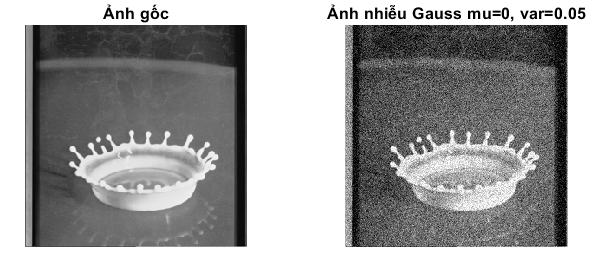
\includegraphics[width=.75\linewidth]{../images/gaussian_noise_matlab.png}
    \caption{Ảnh nhiễu Gauss tạo từ MATLAB}
    \label{fig:gaussian_noise_matlab}
\end{figure}

Nếu không cung cấp thêm tham số, mặc định MATLAB sẽ tạo nhiễu Gauss trắng với trung bình $\mu = 0$ và phương sai hay công suất nhiễu $\sigma^2 = 0.01$.

\subsubsection{Lọc ảnh nhiễu Gauss bằng Python trên Raspberry Pi 3}

Với Python trên Raspberry Pi 3, ta lọc ảnh bằng bộ lọc Wiener với hàm \texttt{wiener()} của thư viện \texttt{scipy.signal}. 
Wiener là bộ lọc thông thấp cho một hình ảnh có giá trị cường độ bị suy hao bởi nhiễu cộng có công suất hằng. 
Với mỗi điểm ảnh, bộ lọc sẽ tìm trung bình và độ lệch chuẩn cục bộ trong một lân cận có kích thước được định sẵn.
Thuật toán của hàm \texttt{wiener()} được mô tả ở hình \ref{fig:wiener_algorithm}.

\begin{figure}[H]
    \centering
    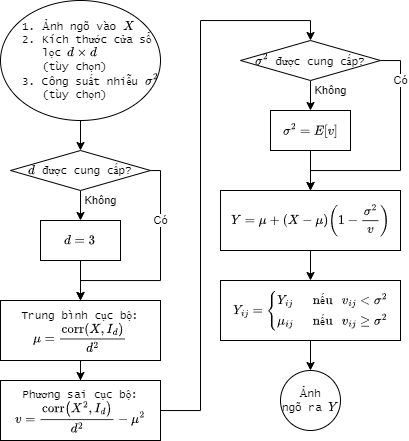
\includegraphics[width=.75\linewidth]{../images/wiener_algorithm.png}
    \caption{Thuật toán của hàm \texttt{wiener()}}
    \label{fig:wiener_algorithm}
\end{figure}

Nếu không cung cấp thêm tham số kích thước bộ lọc và công suất nhiễu,
mặc định hàm \texttt{scipy.signal.wiener()} sẽ:
\begin{itemize}
    \item Chọn kích thước cửa sổ lọc là $3 \times 3$;
    \item Ước lượng công suất nhiễu.
\end{itemize}

Tuy nhiên, cho tới phiên bản Scipy 1.13, hàm \texttt{wiener()} không trả về giá trị được ước lượng của công suất.
Do đó ta tiến hành chỉnh sửa lại mã nguồn của hàm này như sau:

\begin{lstlisting}[language=Python]
from scipy.signal import correlate

def wiener(im, mysize=None, noise=None):
    im = np.asarray(im)
    if mysize is None:
        mysize = [3] * im.ndim
    mysize = np.asarray(mysize)
    if mysize.shape == ():
        mysize = np.repeat(mysize.item(), im.ndim)

    # Uoc luong trung binh cuc bo
    lMean = correlate(im, np.ones(mysize), 'same') / np.prod(mysize, axis=0)

    # Uoc luong phuong sai cuc bo
    lVar = (correlate(im ** 2, np.ones(mysize), 'same') /
            np.prod(mysize, axis=0) - lMean ** 2)

    # Uoc luong cong suat nhieu neu can
    if noise is None:
        noise = np.mean(np.ravel(lVar), axis=0)

    res = (im - lMean)
    res *= (1 - noise / lVar)
    res += lMean
    out = np.where(lVar < noise, lMean, res)

    return [out, noise]
\end{lstlisting}


Ta tiến hành thí nghiệm với hai trường hợp:
\begin{enumerate}
    \item (Mặc định) Không cung cấp tham số công suất nhiễu để phần mềm tự ước lượng giá trị này.
    \item Cung cấp trước tham số nhiễu ($\sigma^2 = 0.01$).
\end{enumerate}

\begin{lstlisting}[language=Python]
import cv2
import numpy as np
import matplotlib.pyplot as plt
import scipy.io

# Doc anh nhieu Gauss
I = cv2.imread('output/gaussian_noise.png', cv2.IMREAD_GRAYSCALE)

# Loc nhieu Gauss bang ham wiener() va luu ket qua
# Truong hop mac dinh (tu uoc luong cong suat nhieu)
[J_default, J_default_noise] = wiener(I, (3,3))
# Cung cap tham so cong suat nhieu var=0.01
[J_var0p01, J_var0p01_noise] = wiener(I, (3,3), 0.01)

# Luu ket qua loc theo dinh dang cua MATLAB
scipy.io.savemat('output/gaussian_denoised_rpi3.mat', 
                 {"J_default": J_default, 
                  "J_default_noise": J_default_noise,
                  "J_var0p01": J_var0p01})
\end{lstlisting}

Kết quả chạy chương trình trên Raspberry Pi 3: 
Chương trình đọc ảnh nhiễu ngõ vào và xuất file \verb|output/gaussian_denoised_rpi3.mat| thành công để đưa vào MATLAB.

\subsubsection{So sánh kết quả với MATLAB}

Ta lọc ảnh bằng bộ lọc Wiener với hàm \texttt{wiener2()} có sẵn của MATLAB. 
Nếu không cung cấp thêm tham số kích thước bộ lọc và công suất nhiễu,
mặc định MATLAB sẽ dùng cửa sổ lọc có kích thước $3 \times 3$, 
và ước lượng công suất nhiễu trước khi thực hiện quá trình lọc.

Tiếp đến, ta vẽ ảnh đã lọc từ MATLAB và từ Raspberry Pi 3, 
đồng thời đánh giá các kết quả này dựa trên sai số bình phương trung bình giữa ảnh đã lọc và ảnh gốc.

\begin{lstlisting}[language=MATLAB]
fig = figure("Position", [0 0 800 500]);
tiledlayout(2,3)

% Doc anh xam goc va hien thi
I = imread('../output/gaussian_orig.png');
nexttile, imshow(I), title('Anh goc')

% Doc anh nhieu Gauss va hien thi
J = imread('../output/gaussian_noise.png');
nexttile, imshow(J), title(["Anh nhieu Gauss", "mu=0, var=0.05"])

% Loc nhieu Gauss bang ham wiener2 co san va hien thi
[K, noise] = wiener2(J);
nexttile, imshow(K), title(["Loc nhieu Gauss", "(MATLAB)"])
imwrite(K, '../output/gaussian_denoised_matlab.png')

% Doc ket qua loc nhieu Gauss tu Raspberry Pi 3 va hien thi
load('../output/gaussian_denoised_rpi3.mat')
L1 = uint8(J1_rpi3);
L2 = uint8(J2_rpi3);
nexttile, imshow(L1), title(["Loc nhieu Gauss", "(RPi 3, mac dinh)"])
imwrite(L1, '../output/gaussian_denoised_rpi3_default.png')
nexttile, imshow(L2), title(["Loc nhieu Gauss", "(RPi 3, var=0.01)"])
imwrite(L2, '../output/gaussian_denoised_rpi3_var_0p01.png')

% Cong suat nhieu uoc luong va sai so trung binh binh phuong
fprintf("Cong suat nhieu uoc luong (truong hop khong cung cap truoc tham so nhieu):\n");
fprintf('MATLAB: %.4f\n', K_noise);
fprintf('Raspberry Pi 3: %.4f\n', J_default_noise);
fprintf('\n');

fprintf('Sai so trung binh binh phuong giua anh goc va anh da loc:\n');
fprintf('MSE (MATLAB): %.4f\n', mse(I, K));
fprintf('MSE (RPi 3, default): %.4f\n', mse(I, L1));
fprintf('MSE (RPi 3, var=0.01): %.4f\n', mse(I, L2));
\end{lstlisting}

\begin{lstlisting}[style=output]
Cong suat nhieu uoc luong (truong hop khong cung cap tham so nhieu)
MATLAB: 0.0105
Raspberry Pi 3: -13035.2815

Sai so binh phuong trung binh giua anh goc va anh da loc:
MSE (MATLAB, mac dinh): 41.1119
MSE (MATLAB, var=0.01): 41.6963
MSE (RPi 3, mac dinh): 66.0795
MSE (RPi 3, var=0.01): 39.0874
\end{lstlisting}

\begin{figure}[H]
    \centering
    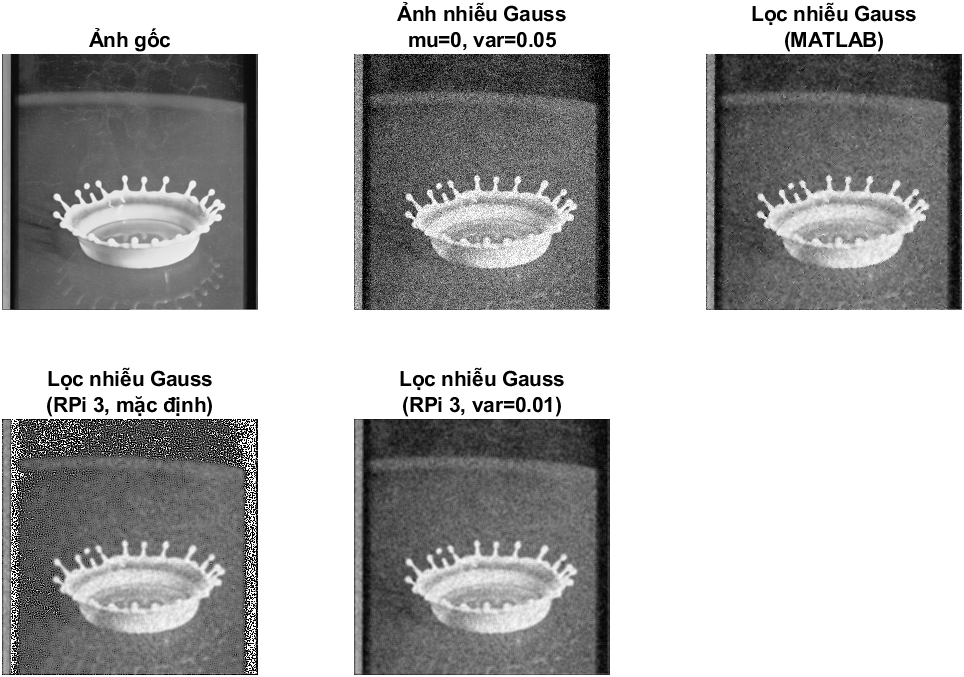
\includegraphics[width=.65\linewidth]{../images/gaussian_compare.png}
    \caption{So sánh kết quả lọc nhiễu Gauss từ Raspberry Pi 3 so với MATLAB}
\end{figure}

\textbf{Nhận xét}: 
\begin{itemize}
    \item \textbf{Trường hợp tự ước lượng công suất nhiễu bằng phần mềm}: 
    MATLAB ước lượng tốt công suất nhiễu (0.0105 so với 0.010), do đó cho kết quả lọc tương đối tốt.
    Trong khi đó, thư viện scipy của Python trên Raspberry Pi 3 ước lượng công suất nhiễu chệch rất nhiều so với công suất nhiễu thực tế (-13035.2815 so với 0.01), do đó cho kết quả lọc tệ hơn.
    Điều này thể hiện ở MSE của MATLAB nhỏ hơn đáng kể ($41.1119 < 66.0795$).

    \item \textbf{Trường hợp cung cấp trước tham số công suất nhiễu}:
    Khi cung cấp trước tham số công suất nhiễu $\sigma^2 = 0.01$, bộ kit lại cho kết quả lọc tốt hơn MATLAB.
    Cụ thể, sai số trung bình bình phương từ kết quả lọc của Raspberry Pi 3 nhỏ hơn so với của MATLAB ($39.0874 < 41.6963$).
\end{itemize}

\subsubsection{So sánh trên toàn bộ dữ liệu}

Thực hiện cùng quy trình thí nghiệm này với các ảnh còn lại trong bộ dữ liệu, ta thu được kết quả sau:

\begin{table}[H]
\centering
\begin{tabular}{|c|cccc|cc|}
\hline
\multirow{3}{*}{\textbf{Filename}} & \multicolumn{4}{c|}{\textbf{Mac dinh}} & \multicolumn{2}{c|}{\textbf{Noise = 0.01}} \\ \cline{2-7} 
 & \multicolumn{2}{c|}{\textbf{MATLAB}} & \multicolumn{2}{c|}{\textbf{RPi3}} & \multicolumn{1}{c|}{\textbf{MATLAB}} & \textbf{RPi3} \\ \cline{2-7} 
 & \multicolumn{1}{c|}{\textbf{Noise}} & \multicolumn{1}{c|}{\textbf{MSE}} & \multicolumn{1}{c|}{\textbf{Noise}} & \textbf{MSE} & \multicolumn{1}{c|}{\textbf{MSE}} & \textbf{MSE} \\ \hline
4.1.01 & \multicolumn{1}{c|}{0.0093} & \multicolumn{1}{c|}{35.2312} & \multicolumn{1}{c|}{-4949.0979} & 73.4121 & \multicolumn{1}{c|}{34.3646} & 32.5127 \\ \hline
4.1.02 & \multicolumn{1}{c|}{0.0078} & \multicolumn{1}{c|}{26.6458} & \multicolumn{1}{c|}{-2057.6920} & 51.8060 & \multicolumn{1}{c|}{24.8055} & 24.9675 \\ \hline
4.1.03 & \multicolumn{1}{c|}{0.0120} & \multicolumn{1}{c|}{40.9004} & \multicolumn{1}{c|}{-19870.1450} & 47.5380 & \multicolumn{1}{c|}{43.2635} & 41.0366 \\ \hline
4.1.04 & \multicolumn{1}{c|}{0.0118} & \multicolumn{1}{c|}{41.7485} & \multicolumn{1}{c|}{-14358.2962} & 68.7183 & \multicolumn{1}{c|}{43.6294} & 41.5368 \\ \hline
4.1.05 & \multicolumn{1}{c|}{0.0119} & \multicolumn{1}{c|}{43.3974} & \multicolumn{1}{c|}{-20863.6106} & 64.4206 & \multicolumn{1}{c|}{45.4044} & 43.3415 \\ \hline
4.1.06 & \multicolumn{1}{c|}{0.0151} & \multicolumn{1}{c|}{50.2411} & \multicolumn{1}{c|}{-20531.3964} & 82.0751 & \multicolumn{1}{c|}{52.6044} & 53.7265 \\ \hline
4.1.07 & \multicolumn{1}{c|}{0.0115} & \multicolumn{1}{c|}{38.3446} & \multicolumn{1}{c|}{-32041.4723} & 46.9728 & \multicolumn{1}{c|}{40.3967} & 37.0458 \\ \hline
4.1.08 & \multicolumn{1}{c|}{0.0119} & \multicolumn{1}{c|}{40.5311} & \multicolumn{1}{c|}{-29350.5579} & 52.3743 & \multicolumn{1}{c|}{42.9729} & 40.1785 \\ \hline
4.2.01 & \multicolumn{1}{c|}{0.0105} & \multicolumn{1}{c|}{41.0319} & \multicolumn{1}{c|}{-12996.8919} & 66.2440 & \multicolumn{1}{c|}{41.6784} & 39.5524 \\ \hline
4.2.03 & \multicolumn{1}{c|}{0.0141} & \multicolumn{1}{c|}{58.9022} & \multicolumn{1}{c|}{-17811.8769} & 73.1133 & \multicolumn{1}{c|}{60.0894} & 62.0433 \\ \hline
4.2.05 & \multicolumn{1}{c|}{0.0139} & \multicolumn{1}{c|}{47.8020} & \multicolumn{1}{c|}{-33459.0209} & 61.9616 & \multicolumn{1}{c|}{50.0903} & 51.1122 \\ \hline
4.2.06 & \multicolumn{1}{c|}{0.0140} & \multicolumn{1}{c|}{47.7164} & \multicolumn{1}{c|}{-19410.9745} & 80.2701 & \multicolumn{1}{c|}{50.0511} & 50.1180 \\ \hline
4.2.07 & \multicolumn{1}{c|}{0.0122} & \multicolumn{1}{c|}{41.9256} & \multicolumn{1}{c|}{-16943.4129} & 67.7821 & \multicolumn{1}{c|}{44.3010} & 42.4176 \\ \hline
5.1.09 & \multicolumn{1}{c|}{0.0111} & \multicolumn{1}{c|}{47.7691} & \multicolumn{1}{c|}{-16796.5722} & 55.9229 & \multicolumn{1}{c|}{48.9364} & 46.7720 \\ \hline
5.1.10 & \multicolumn{1}{c|}{0.0157} & \multicolumn{1}{c|}{58.4775} & \multicolumn{1}{c|}{-21107.4482} & 78.2653 & \multicolumn{1}{c|}{60.2243} & 62.2025 \\ \hline
5.1.11 & \multicolumn{1}{c|}{0.0109} & \multicolumn{1}{c|}{40.4260} & \multicolumn{1}{c|}{-38016.1132} & 48.0063 & \multicolumn{1}{c|}{41.4247} & 40.9802 \\ \hline
5.1.12 & \multicolumn{1}{c|}{0.0128} & \multicolumn{1}{c|}{45.3810} & \multicolumn{1}{c|}{-36891.2660} & 63.1316 & \multicolumn{1}{c|}{46.6671} & 49.0570 \\ \hline
5.1.13 & \multicolumn{1}{c|}{0.0244} & \multicolumn{1}{c|}{111.5673} & \multicolumn{1}{c|}{-50761.9816} & 117.1397 & \multicolumn{1}{c|}{105.4671} & 116.2954 \\ \hline
5.1.14 & \multicolumn{1}{c|}{0.0129} & \multicolumn{1}{c|}{51.0761} & \multicolumn{1}{c|}{-12304.1432} & 74.2564 & \multicolumn{1}{c|}{53.0954} & 52.5074 \\ \hline
\end{tabular}
\end{table}

\begin{table}[H]
\centering
\begin{tabular}{|c|cccc|cc|}
\hline
\multirow{3}{*}{\textbf{Filename}} & \multicolumn{4}{c|}{\textbf{Mac dinh}} & \multicolumn{2}{c|}{\textbf{Noise = 0.01}} \\ \cline{2-7} 
 & \multicolumn{2}{c|}{\textbf{MATLAB}} & \multicolumn{2}{c|}{\textbf{RPi3}} & \multicolumn{1}{c|}{\textbf{MATLAB}} & \textbf{RPi3} \\ \cline{2-7} 
 & \multicolumn{1}{c|}{\textbf{Noise}} & \multicolumn{1}{c|}{\textbf{MSE}} & \multicolumn{1}{c|}{\textbf{Noise}} & \textbf{MSE} & \multicolumn{1}{c|}{\textbf{MSE}} & \textbf{MSE} \\ \hline
5.2.08 & \multicolumn{1}{c|}{0.0126} & \multicolumn{1}{c|}{46.9440} & \multicolumn{1}{c|}{-16293.7235} & 61.2985 & \multicolumn{1}{c|}{48.6607} & 47.5992 \\ \hline
5.2.09 & \multicolumn{1}{c|}{0.0167} & \multicolumn{1}{c|}{57.8253} & \multicolumn{1}{c|}{-33225.4572} & 67.1652 & \multicolumn{1}{c|}{58.4314} & 62.7763 \\ \hline
5.2.10 & \multicolumn{1}{c|}{0.0139} & \multicolumn{1}{c|}{56.6113} & \multicolumn{1}{c|}{-15226.0315} & 81.3532 & \multicolumn{1}{c|}{57.9642} & 59.3643 \\ \hline
5.3.01 & \multicolumn{1}{c|}{0.0125} & \multicolumn{1}{c|}{43.6389} & \multicolumn{1}{c|}{-10769.8362} & 65.7852 & \multicolumn{1}{c|}{45.0282} & 46.3524 \\ \hline
5.3.02 & \multicolumn{1}{c|}{0.0125} & \multicolumn{1}{c|}{51.5868} & \multicolumn{1}{c|}{-7596.2661} & 73.6383 & \multicolumn{1}{c|}{53.2986} & 52.7383 \\ \hline
7.1.01 & \multicolumn{1}{c|}{0.0108} & \multicolumn{1}{c|}{46.0228} & \multicolumn{1}{c|}{-11980.7130} & 55.3913 & \multicolumn{1}{c|}{46.9575} & 44.1631 \\ \hline
7.1.02 & \multicolumn{1}{c|}{0.0115} & \multicolumn{1}{c|}{39.7870} & \multicolumn{1}{c|}{-30876.5094} & 41.7975 & \multicolumn{1}{c|}{41.7456} & 39.2065 \\ \hline
7.1.03 & \multicolumn{1}{c|}{0.0110} & \multicolumn{1}{c|}{44.2193} & \multicolumn{1}{c|}{-17975.5355} & 52.1784 & \multicolumn{1}{c|}{45.4040} & 42.7549 \\ \hline
7.1.04 & \multicolumn{1}{c|}{0.0104} & \multicolumn{1}{c|}{44.5998} & \multicolumn{1}{c|}{-14420.1253} & 52.3886 & \multicolumn{1}{c|}{45.1665} & 42.0101 \\ \hline
7.1.05 & \multicolumn{1}{c|}{0.0117} & \multicolumn{1}{c|}{50.1191} & \multicolumn{1}{c|}{-12179.5757} & 66.0205 & \multicolumn{1}{c|}{51.6857} & 50.0475 \\ \hline
7.1.06 & \multicolumn{1}{c|}{0.0113} & \multicolumn{1}{c|}{49.9953} & \multicolumn{1}{c|}{-8977.6643} & 67.0978 & \multicolumn{1}{c|}{51.0894} & 49.2660 \\ \hline
7.1.07 & \multicolumn{1}{c|}{0.0111} & \multicolumn{1}{c|}{49.9211} & \multicolumn{1}{c|}{-11985.2352} & 55.9454 & \multicolumn{1}{c|}{51.1771} & 48.5177 \\ \hline
7.1.08 & \multicolumn{1}{c|}{0.0104} & \multicolumn{1}{c|}{43.1070} & \multicolumn{1}{c|}{-16489.4790} & 46.8678 & \multicolumn{1}{c|}{43.7457} & 41.0177 \\ \hline
7.1.09 & \multicolumn{1}{c|}{0.0113} & \multicolumn{1}{c|}{49.7544} & \multicolumn{1}{c|}{-16676.8104} & 64.2958 & \multicolumn{1}{c|}{51.0697} & 49.2057 \\ \hline
7.1.10 & \multicolumn{1}{c|}{0.0108} & \multicolumn{1}{c|}{45.2453} & \multicolumn{1}{c|}{-14688.9014} & 53.0281 & \multicolumn{1}{c|}{46.3296} & 42.9850 \\ \hline
7.2.01 & \multicolumn{1}{c|}{0.0073} & \multicolumn{1}{c|}{24.0014} & \multicolumn{1}{c|}{-1706.1240} & 70.5824 & \multicolumn{1}{c|}{21.1649} & 19.9642 \\ \hline
boat.512 & \multicolumn{1}{c|}{0.0131} & \multicolumn{1}{c|}{47.6931} & \multicolumn{1}{c|}{-18492.6913} & 64.2792 & \multicolumn{1}{c|}{49.8632} & 50.1183 \\ \hline
gray21.512 & \multicolumn{1}{c|}{0.0092} & \multicolumn{1}{c|}{39.9605} & \multicolumn{1}{c|}{-21425.8306} & 67.2078 & \multicolumn{1}{c|}{38.8942} & 37.1617 \\ \hline
house & \multicolumn{1}{c|}{0.0140} & \multicolumn{1}{c|}{49.9374} & \multicolumn{1}{c|}{-27705.0110} & 64.0971 & \multicolumn{1}{c|}{52.1837} & 52.2799 \\ \hline
ruler.512 & \multicolumn{1}{c|}{0.0269} & \multicolumn{1}{c|}{139.0348} & \multicolumn{1}{c|}{-47894.1489} & 147.9325 & \multicolumn{1}{c|}{119.3403} & 146.8871 \\ \hline
\end{tabular}
\end{table}

\textbf{Nhận xét}: 

\begin{center}
    \textbf{Trường hợp tự ước lượng công suất nhiễu bằng phần mềm}:
\end{center}

MATLAB ước lượng tốt công suất nhiễu (Hình \ref{fig:hist_gaussian_compare_matlab_noise}), 
do đó cho kết quả lọc tương đối tốt.
Trong khi đó, thư viện scipy của Python trên Raspberry Pi 3 ước lượng công suất nhiễu chệch rất nhiều so với công suất nhiễu thực tế.

\begin{figure}[H]
    \centering
    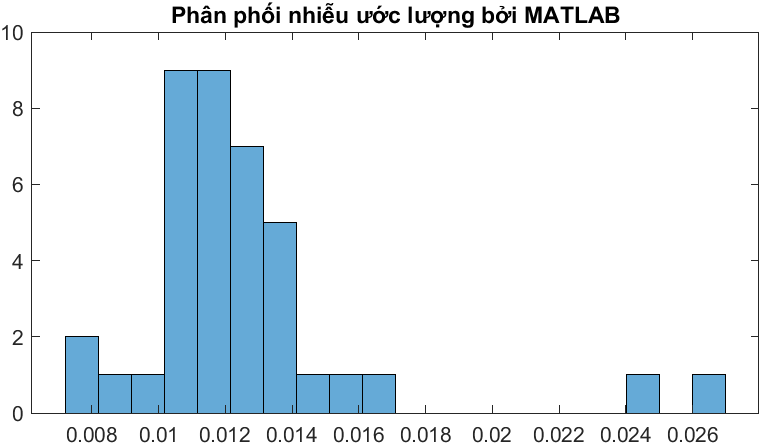
\includegraphics[width=.75\linewidth]{../images/hist_gaussian_compare_matlab_noise.png}
    \caption{Phân phối nhiễu ước lượng bởi MATLAB}
    \label{fig:hist_gaussian_compare_matlab_noise}
\end{figure}

Về mặt sai số, kết quả lọc từ MATLAB cũng có xu hướng cho sai số bình phương trung bình 
thấp hơn so với kết quả từ Python trên kit Raspberry Pi 3 (Hình \ref{fig:hist_gaussian_compare_default_mse}).

\begin{figure}[H]
    \centering
    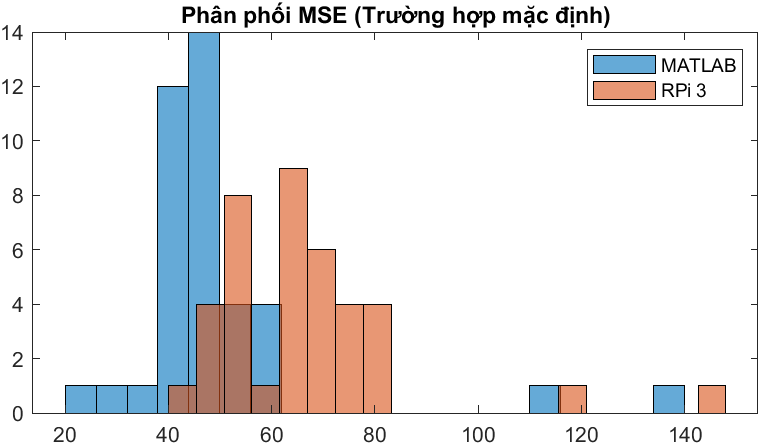
\includegraphics[width=.75\linewidth]{../images/hist_gaussian_compare_default_mse.png}
    \caption{Phân phối MSE (Trường hợp mặc định)}
    \label{fig:hist_gaussian_compare_default_mse}
\end{figure}

\begin{center}
    \textbf{Trường hợp cung cấp trước tham số công suất nhiễu}:
\end{center}

Khi cung cấp trước tham số công suất nhiễu $\sigma^2 = 0.01$, 
bộ kit lại cho kết quả lọc tốt hơn MATLAB.
Phân phối MSE cho Raspberry Pi 3 có xu hướng nhỏ hơn so với của MATLAB (Hình \ref{fig:hist_gaussian_compare_var0p01_mse}).
Trong 39 ảnh được dùng để so sánh giữa MATLAB và Python trên Raspberry Pi 3, có đến gần 2/3 tổng số ảnh mà bộ kit cho kết quả lọc tốt hơn (Hình \ref{fig:pie_gaussian_compare_var0p01_mse})

\begin{figure}[H]
    \centering
    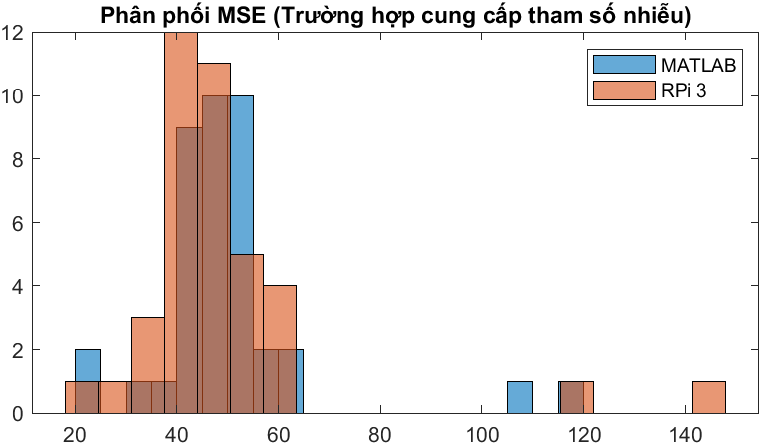
\includegraphics[width=.75\linewidth]{../images/hist_gaussian_compare_var0p01_mse.png}
    \caption{Phân phối MSE (Trường hợp cung cấp tham số nhiễu)}
    \label{fig:hist_gaussian_compare_var0p01_mse}
\end{figure}

\begin{figure}[H]
    \centering
    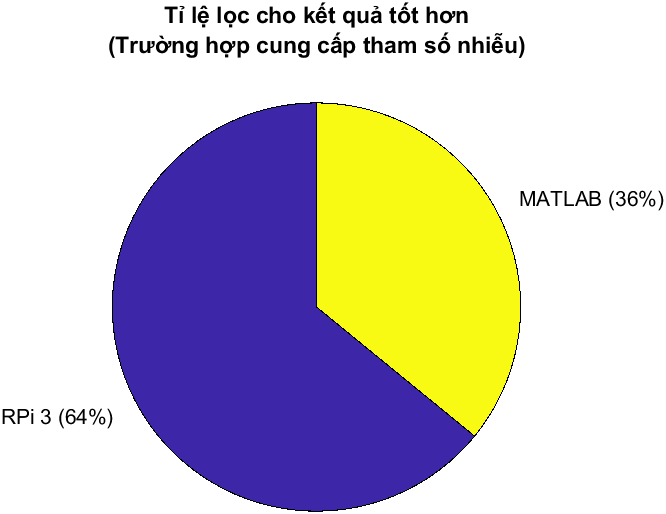
\includegraphics[width=.75\linewidth]{../images/pie_gaussian_compare_var0p01_mse.png}
    \caption{Tỉ lệ lọc cho kết quả tốt hơn (Trường hợp cung cấp tham số nhiễu)}
    \label{fig:pie_gaussian_compare_var0p01_mse}
\end{figure}